\section{Clustering complexity on the hypercube}
\subsection{Brief recap on computational complexity}
Recall that $\mathcal{P}$ is the class of problems that can be \textit{solved} in polynomial time by a deterministic Turing machine, and $\mathcal{NP}$ is the class of problems for which a solution can be \textit{verified} in polynomial time by a deterministic Turing machine. The class $\mathcal{NP}$ is the class of problems that can be solved non-deterministically in polynomial time. A problem is:
\begin{itemize}
    \item \textbf{$\mathcal{NP}$-complete} if it is in $\mathcal{NP}$ and every problem in $\mathcal{NP}$ can be reduced to it in polynomial time
    \item \textbf{$\mathcal{NP}$-hard} if there is a $\mathcal{NP}$-complete problem that can be reduced to it in polynomial time
\end{itemize}
An example of an $\mathcal{NP}$-complete problem is the Boolean satisfiability problem (SAT), which is the problem of determining whether a given Boolean formula can be satisfied by assigning truth values to its variables. If it could be solved in polynomial time, then every problem in $\mathcal{NP}$ could be solved in polynomial time because every problem in $\mathcal{NP}$ can be reduced to SAT in polynomial time.

\subsection{Clustering complexity}
In this section, we briefly review some results on clustering complexity and then prove that the hypercube clustering decision problem is in general NP-complete. 

% missing some details

A graph is cubical if it is the subgraph of some hypercube $\mathbb{H}^d$ for some $d$. Although deciding whether a graph is cubical is NP-complete, there is a theorem providing a necessary and sufficient condition for a graph to be cubical. A graph $G(V,E)$ is cubical and embeddable in $\mathbb{H}^d$ if and only if it is possible to color the edges of $G$ with $d$ colors such that:
\begin{enumerate}
    \item All edges incident with a common vertex are of different color
    \item In each path of $G$, there is some color that appears an odd number of times
    \item In each cycle of $G$, no color appears an odd number of times
\end{enumerate} 
\begin{theorem}
    Consider the following hypercube clustering problem:
    \begin{itemize}
        \item \textbf{Input:} $m$ binary vectors $x_1, \dots, x_m$ of length $n$ and an integer $k$
        \item \textbf{Output:} $k$ binary vectors $c_1, \dots, c_k$ of length $n$ (the centroids) and a function $f$ from $\{x_1, \dots, x_m\}$ to $\{c_1, \dots, c_k\}$ that minimizes the distortion 
        \[
            E = \sum_{t=1}^m \Delta(x_t, f(x_t))    
        \]
        Where $\Delta$ is Hamming distance.
    \end{itemize}
    The hypercube clustering decision problem $\mathcal{NP}$-hard when $k \sim m^\epsilon$ $(\epsilon > 0)$
\end{theorem}
\begin{proof}
    To sketch the reduction, we start from the problem of clustering $m$ points in the plane $\mathbb{R}^2$ using cluster centroids and the $L_1$ distance, which is $\mathcal{NP}$-complete by reduction from 3-SAT when $k \sim m^\epsilon$ $(\epsilon > 0)$. Without any loss of generality, we can assume that the points in these problems lie on the vertices of a square lattice. Using the theorem in Havel and Moravek, one can show that a $n \times m$ square lattice in the plane can be embedded in a hypercube $\mathbb{H}^{m+n}$. 
    Example:
    \begin{multicols}{2}
    \begin{center}
                % 4x2 Lattice with different shaped lines
        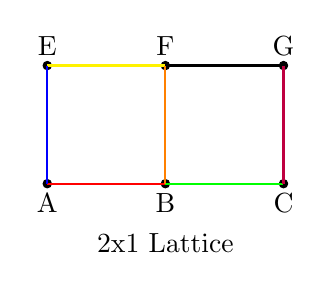
\begin{tikzpicture}[scale=1.5]
            % Draw the grid points
            \filldraw[black] (0,0) circle (1pt) node[anchor=north] {A};
            \filldraw[black] (1,0) circle (1pt) node[anchor=north] {B};
            \filldraw[black] (2,0) circle (1pt) node[anchor=north] {C};
            %\filldraw[black] (3,0) circle (1pt) node[anchor=north] {D};

            \filldraw[black] (0,1) circle (1pt) node[anchor=south] {E};
            \filldraw[black] (1,1) circle (1pt) node[anchor=south] {F};
            \filldraw[black] (2,1) circle (1pt) node[anchor=south] {G};
            %\filldraw[black] (3,1) circle (1pt) node[anchor=south] {H};

            % Connect the points with different line styles
            \draw[red,thick] (0,0) -- (1,0); % Solid line
            \draw[green,thick] (1,0) -- (2,0); % Dashed line
            %\draw[dotted, thick] (2,0) -- (3,0); % Dotted line
            \draw[yellow,thick] (0,1) -- (1,1); % Dash-dot line
            \draw[thick] (1,1) -- (2,1); % Solid line
            %\draw[dashed, thick] (2,1) -- (3,1); % Dashed line
            \draw[blue,thick] (0,0) -- (0,1); % Dotted line
            \draw[orange,thick] (1,0) -- (1,1); % Dash-dot line
            \draw[purple,thick] (2,0) -- (2,1); % Solid line
            %\draw[dashed, thick] (3,0) -- (3,1); % Dashed line

            % Label the lattice
            \node at (1, -0.5) {2x1 Lattice};
        \end{tikzpicture}
    \end{center}
    \columnbreak
    \begin{center}
                % 3D Cube with connections following the lattice pattern
        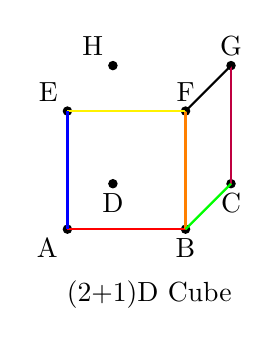
\begin{tikzpicture}[scale=1.5]
            % Draw the vertices of the cube (front and back face)
            \filldraw[black] (0,0,0) circle (1pt) node[anchor=north] {D}; % Front bottom left
            \filldraw[black] (1,0,0) circle (1pt) node[anchor=north] {C}; % Front bottom right
            \filldraw[black] (0,1,0) circle (1pt) node[anchor=south east] {H}; % Front top left
            \filldraw[black] (1,1,0) circle (1pt) node[anchor=south] {G}; % Front top right

            \filldraw[black] (0,0,1) circle (1pt) node[anchor=north east] {A}; % Back bottom left
            \filldraw[black] (1,0,1) circle (1pt) node[anchor=north] {B}; % Back bottom right
            \filldraw[black] (0,1,1) circle (1pt) node[anchor=south east] {E}; % Back top left
            \filldraw[black] (1,1,1) circle (1pt) node[anchor=south] {F}; % Back top right

            % Connect the vertices with corresponding line styles from the lattice
            %\draw[green,thick] (0,0,0) -- (1,0,0); % Solid line (A-B)
            \draw[purple,thick] (1,0,0) -- (1,1,0); % Dashed line (B-F)
            %\draw[purple,thick] (0,1,0) -- (1,1,0); % Dotted line (E-F)
            %\draw[green,thick] (0,0,0) -- (0,1,0); % Dash-dot line (A-E)

            \draw[red,thick] (0,0,1) -- (1,0,1); % Solid line (C-D)
            \draw[orange,thick] (1,0,1) -- (1,1,1); % Dashed line (D-H)
            \draw[yellow,thick] (0,1,1) -- (1,1,1); % Dotted line (G-H)
            \draw[blue,thick] (0,0,1) -- (0,1,1); % Dash-dot line (C-G)

            % Connect the front and back face vertices
            %\draw[blue,thick] (0,0,0) -- (0,0,1); % Solid line (A-C)
            \draw[green,thick] (1,0,0) -- (1,0,1); % Dashed line (B-D)
            %\draw[blue,thick] (0,1,0) -- (0,1,1); % Dotted line (E-G)
            \draw[,thick] (1,1,0) -- (1,1,1); % Dash-dot line (F-H)

            % Label the cube
            \node at (0.5, -0.75, 0.5) {(2+1)D Cube};
        \end{tikzpicture}        
    \end{center}

        \end{multicols}
    
    

    It is easy to check that the $L_1$ or Manhattan distance between any two points on the square lattice is equal to the corresponding Hamming distance in $\mathbb{H}^{m+n}$. This polynomial reduction completes the proof that if the number of cluster satisfies $k = 2^p \sim m^\epsilon$ or equivalently $p \sim \epsilon \log_2 m \sim C \log n$, then the hypercube clustering problem associated with the Boolean autoencoder is $\mathcal{NP}$-hard and the corresponding decision problem is $\mathcal{NP}$-complete. If the numbers $k$ of clusters is fixed and the centroids must belong to the training set, there are only $\binom{m}{k} \sim m^k$ possible choices for the centroids inducing the corresponding Voronoi clusters. This yields a trivial, albeit not efficient, polynomial time algorithm. When the centroids are not required to be in the training set, we conjecture also the existence of polynomial time algorithms by adapting the corresponing theorems in Euclidean space. 
\end{proof}

